% 若编译失败,且生成 .synctex(busy) 辅助文件,可能有两个原因:
% 1. 需要插入的图片不存在:Ctrl + F 搜索 'figure' 将这些代码注释/删除掉即可
% 2. 路径/文件名含中文或空格:更改路径/文件名即可

% --------------------- 文章宏包及相关设置 --------------------- %
% >> ------------------ 文章宏包及相关设置 ------------------ << %
% 设定文章类型与编码格式
\documentclass[UTF8]{report}		


% 自定义宏定义
    \def\N{\mathbb{N}}
    \def\F{\mathbb{F}}
    \def\Z{\mathbb{Z}}
    \def\Q{\mathbb{Q}}
    \def\R{\mathbb{R}}
    \def\C{\mathbb{C}}
    \def\T{\mathbb{T}}
    \def\S{\mathbb{S}}
    \def\A{\mathbb{A}}
    \def\I{\mathscr{I}}
    \def\d{\mathrm{d}}
    \def\p{\partial}


% 导入基本宏包
    \usepackage[UTF8]{ctex}     % 设置文档为中文语言
    \usepackage[colorlinks, linkcolor=blue, anchorcolor=blue, citecolor=blue, urlcolor=blue]{hyperref}  % 宏包:自动生成超链接 (此宏包与标题中的数学环境冲突)
    % \usepackage{docmute}    % 宏包:子文件导入时自动去除导言区,用于主/子文件的写作方式,\include{./51单片机笔记}即可。注:启用此宏包会导致.tex文件capacity受限。
    \usepackage{amsmath}    % 宏包:数学公式
    \usepackage{mathrsfs}   % 宏包:提供更多数学符号
    \usepackage{amssymb}    % 宏包:提供更多数学符号
    \usepackage{pifont}     % 宏包:提供了特殊符号和字体
    \usepackage{extarrows}  % 宏包:更多箭头符号 
    \usepackage{multicol}   % 宏包:支持多栏 

% 文章页面margin设置
    \usepackage[a4paper]{geometry}
        \geometry{top=1in}
        \geometry{bottom=1in}
        \geometry{left=0.75in}
        \geometry{right=0.75in}   % 设置上下左右页边距
        \geometry{marginparwidth=1.75cm}    % 设置边注距离(注释、标记等)

% 配置数学环境
    \usepackage{amsthm} % 宏包:数学环境配置
    % theorem-line 环境自定义
        \newtheoremstyle{MyLineTheoremStyle}% <name>
            {11pt}% <space above>
            {11pt}% <space below>
            {}% <body font> 使用默认正文字体
            {}% <indent amount>
            {\bfseries}% <theorem head font> 设置标题项为加粗
            {:}% <punctuation after theorem head>
            {.5em}% <space after theorem head>
            {\textbf{#1}\thmnumber{#2}\ \ (\,\textbf{#3}\,)}% 设置标题内容顺序
        \theoremstyle{MyLineTheoremStyle} % 应用自定义的定理样式
        \newtheorem{LineTheorem}{Theorem.\,}
    % theorem-block 环境自定义
        \newtheoremstyle{MyBlockTheoremStyle}% <name>
            {11pt}% <space above>
            {11pt}% <space below>
            {}% <body font> 使用默认正文字体
            {}% <indent amount>
            {\bfseries}% <theorem head font> 设置标题项为加粗
            {:\\ \indent}% <punctuation after theorem head>
            {.5em}% <space after theorem head>
            {\textbf{#1}\thmnumber{#2}\ \ (\,\textbf{#3}\,)}% 设置标题内容顺序
        \theoremstyle{MyBlockTheoremStyle} % 应用自定义的定理样式
        \newtheorem{BlockTheorem}[LineTheorem]{Theorem.\,} % 使用 LineTheorem 的计数器
    % definition 环境自定义
        \newtheoremstyle{MySubsubsectionStyle}% <name>
            {11pt}% <space above>
            {11pt}% <space below>
            {}% <body font> 使用默认正文字体
            {}% <indent amount>
            {\bfseries}% <theorem head font> 设置标题项为加粗
            {:\\ \indent}% <punctuation after theorem head>
            {0pt}% <space after theorem head>
            {\textbf{#3}}% 设置标题内容顺序
        \theoremstyle{MySubsubsectionStyle} % 应用自定义的定理样式
        \newtheorem{definition}{}

%宏包:有色文本框(proof环境)及其设置
    \usepackage[dvipsnames,svgnames]{xcolor}    %设置插入的文本框颜色
    \usepackage[strict]{changepage}     % 提供一个 adjustwidth 环境
    \usepackage{framed}     % 实现方框效果
        \definecolor{graybox_color}{rgb}{0.95,0.95,0.96} % 文本框颜色。修改此行中的 rgb 数值即可改变方框纹颜色,具体颜色的rgb数值可以在网站https://colordrop.io/ 中获得。(截止目前的尝试还没有成功过,感觉单位不一样)(找到喜欢的颜色,点击下方的小眼睛,找到rgb值,复制修改即可)
        \newenvironment{graybox}{%
        \def\FrameCommand{%
        \hspace{1pt}%
        {\color{gray}\small \vrule width 2pt}%
        {\color{graybox_color}\vrule width 4pt}%
        \colorbox{graybox_color}%
        }%
        \MakeFramed{\advance\hsize-\width\FrameRestore}%
        \noindent\hspace{-4.55pt}% disable indenting first paragraph
        \begin{adjustwidth}{}{7pt}%
        \vspace{2pt}\vspace{2pt}%
        }
        {%
        \vspace{2pt}\end{adjustwidth}\endMakeFramed%
        }

% 外源代码插入设置
    % matlab 代码插入设置
    \usepackage{matlab-prettifier}
        \lstset{
            style=Matlab-editor,  % 继承matlab代码颜色等
        }
    \usepackage[most]{tcolorbox} % 引入tcolorbox包 
    \usepackage{listings} % 引入listings包
        \tcbuselibrary{listings, skins, breakable}
        \lstdefinestyle{matlabstyle}{
            language=Matlab,
            basicstyle=\small,
            breakatwhitespace=false,
            breaklines=true,
            captionpos=b,
            keepspaces=true,
            numbers=left,
            numbersep=15pt,
            showspaces=false,
            showstringspaces=false,
            showtabs=false,
            tabsize=2
        }
        \newtcblisting{matlablisting}{
            arc=0pt,
            top=0pt,
            bottom=0pt,
            left=1mm,
            listing only,
            listing style=matlabstyle,
            breakable,
            colback=white   % 选一个合适的颜色
        }

% table 支持
    \usepackage{booktabs}   % 宏包:三线表
    \usepackage{tabularray} % 宏包:表格排版
    \usepackage{longtable}  % 宏包:长表格

% figure 设置
    \usepackage{graphicx}  % 支持 jpg, png, eps, pdf 图片 
    \usepackage{svg}       % 支持 svg 图片
        \svgsetup{
            % 指向 inkscape.exe 的路径
            inkscapeexe = D:/aa_my_apps_main/Inkscape/bin/inkscape.exe, 
            % 一定程度上修复导入后图片文字溢出几何图形的问题
            inkscapelatex = false                 
        }

% 图表进阶设置
    \usepackage{caption}    % 图注、表注
        \captionsetup[figure]{name=图}  
        \captionsetup[table]{name=表}
        \captionsetup{labelfont=bf, font=small}
    \usepackage{float}     % 图表位置浮动设置 

% 圆圈序号自定义
    \newcommand*\circled[1]{\tikz[baseline=(char.base)]{\node[shape=circle,draw,inner sep=0.8pt, line width = 0.03em] (char) {\small \bfseries #1};}}   % TikZ solution

% 列表设置
    \usepackage{enumitem}   % 宏包:列表环境设置
        \setlist[enumerate]{itemsep=0pt, parsep=0pt, topsep=0pt, partopsep=0pt, leftmargin=3.5em} 
        \setlist[itemize]{itemsep=0pt, parsep=0pt, topsep=0pt, partopsep=0pt, leftmargin=3.5em}
        \newlist{circledenum}{enumerate}{1} % 创建一个新的枚举环境  
        \setlist[circledenum,1]{  
            label=\protect\circled{\arabic*}, % 使用 \arabic* 来获取当前枚举计数器的值,并用 \circled 包装它  
            ref=\arabic*, % 如果需要引用列表项,这将决定引用格式(这里仍然使用数字)
            itemsep=0pt, parsep=0pt, topsep=0pt, partopsep=0pt, leftmargin=3.5em
        }  

% 其它设置
    % 脚注设置
        \renewcommand\thefootnote{\ding{\numexpr171+\value{footnote}}}
    % 参考文献引用设置
        \bibliographystyle{unsrt}   % 设置参考文献引用格式为unsrt
        \newcommand{\upcite}[1]{\textsuperscript{\cite{#1}}}     % 自定义上角标式引用
    % 文章序言设置
        \newcommand{\cnabstractname}{序言}
        \newenvironment{cnabstract}{%
            \par\Large
            \noindent\mbox{}\hfill{\bfseries \cnabstractname}\hfill\mbox{}\par
            \vskip 2.5ex
            }{\par\vskip 2.5ex}

% 文章默认字体设置
\usepackage{fontspec}   % 宏包:字体设置
    \setmainfont{SimSun}    % 设置中文字体为宋体字体
    \setmainfont{Times New Roman} % 设置英文字体为Times New Roman

% 各级标题自定义设置
\usepackage{titlesec}   
\titleformat{\chapter}[hang]{\normalfont\huge\bfseries\centering}{第\,\thechapter\,章}{20pt}{}
\titlespacing*{\chapter}{0pt}{-20pt}{20pt} % 控制上方空白的大小
% section标题自定义设置 
\titleformat{\section}[hang]{\normalfont\Large\bfseries}{§\,\thesection\,}{8pt}{}
% subsubsection标题自定义设置
%\titleformat{\subsubsection}[hang]{\normalfont\bfseries}{}{8pt}{}

% --------------------- 文章宏包及相关设置 --------------------- %
% >> ------------------ 文章宏包及相关设置 ------------------ << %

% ------------------------ 文章信息区 ------------------------ %
% ------------------------ 文章信息区 ------------------------ %
% 页眉页脚设置
    \usepackage{fancyhdr}   %宏包:页眉页脚设置
        \pagestyle{fancy}
        \fancyhf{}
        \cfoot{\thepage}
        \renewcommand\headrulewidth{1pt}
        \renewcommand\footrulewidth{0pt}
        \lhead{2024.8-2025.1}
        \chead{Notes of Circuit Theory}    
        \rhead{dingyi233@mails.ucas.ac.cn}

%文档信息设置
    \title{电路原理笔记\\ Notes of Circuit Theory}
    \author{丁毅\\ \footnotesize 中国科学院大学,北京 100049\\ Yi Ding \\ \footnotesize University of Chinese Academy of Sciences, Beijing 100049, China}
    \date{\footnotesize 2024.8 -- 2025.1}
% ------------------------ 文章信息区 ------------------------ %
% ------------------------ 文章信息区 ------------------------ %

% 开始编辑文章

\begin{document} 
\zihao{5}           % 设置全文字号大小

% ------------------------ 封面序言与目录 ------------------------ %
% >> --------------------- 封面序言与目录 --------------------- << %
% 封面
    \maketitle\newpage  
    \pagenumbering{Roman} % 页码为大写罗马数字
    \thispagestyle{fancy}   % 显示页码、页眉等

% 序言
    \begin{cnabstract}\normalsize 
        本文为笔者本科时的电路原理笔记(Notes of Circuit Theory, 2024.9-2025.1)。由于个人学识浅陋,认识有限,文中难免有不妥甚至错误之处,望读者不吝指正,在此感谢。\par
        我的邮箱是 dingyi233@mails.ucas.ac.cn。
    \end{cnabstract}
    \addcontentsline{toc}{chapter}{序言} % 手动添加为目录

% 目录
    \setcounter{tocdepth}{2}                % 目录深度(为1时显示到section)
    \tableofcontents                        % 目录页
    \addcontentsline{toc}{chapter}{目录}    % 手动添加此页为目录
    \thispagestyle{fancy}                   % 显示页码、页眉等 

% 收尾工作
    \newpage    
    \pagenumbering{arabic} 


% >> --------------------- 封面序言与目录 --------------------- << %
% ------------------------ 封面序言与目录 ------------------------ %

\chapter{绪论}\thispagestyle{fancy}

本章首先介绍几个有关电路的基本问题,然后介绍电路中相关物理量的定义,再简单介绍电路在信号处理与能量处理方面的应用,最后讨论电路的分类。本章是所有后续章节的共同基础。

\section{电路}
一般来讲,电路的研究内容分为电路分析、电路综合,分别对应电路研究的正问题(已知电路求电路的解)和逆问题(已知解求电路结构参数),本课程的重点在电路分析,对电路综合不深入探讨。

\begin{figure}[H]\centering
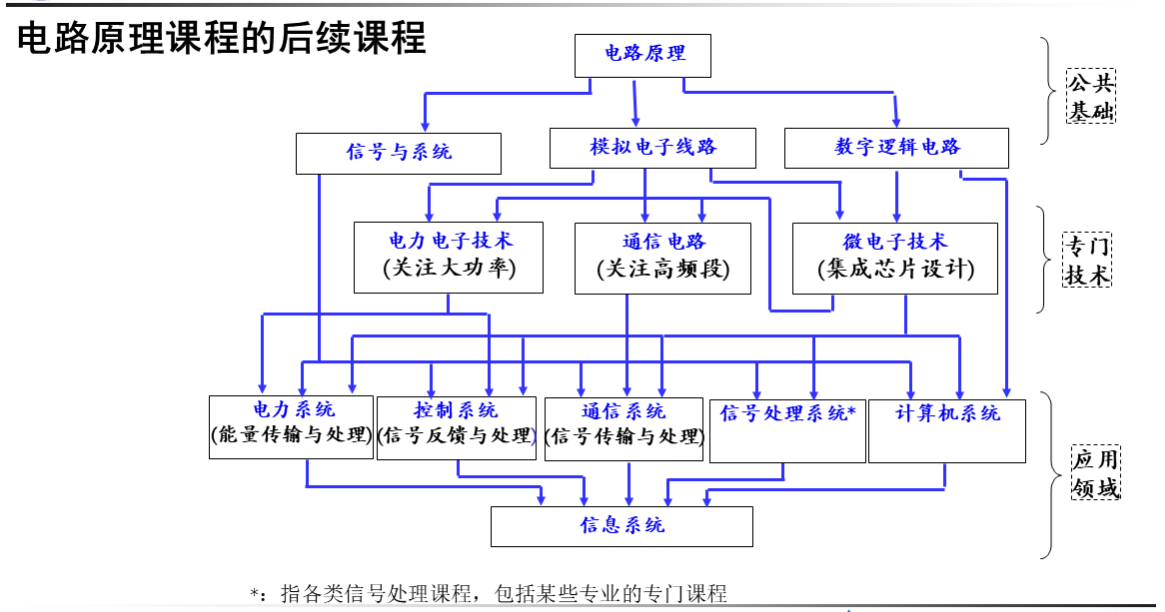
\includegraphics[width=0.5\textwidth]{assets/11b7879b24f71ddbf3e5316424203201.png}
\caption{\textbf{电路原理与其他电类主要课程的联系}}\label{电路原理与其他电类主要课程的联系}
\end{figure}

有些电路原理课程习惯用大写英文字母表示不随时间变化的常量,用小写英文字母表示随时间变化的量。在本笔记中,时变量(非恒定量)、瞬时量、微元量均用小写表示,其它情况一般用大写。



\section{电流、电压和电势}

电势(电位,potential):选定参考点(reference point)后,电路中某一点的电势,用 $\varphi$ 表示。如果不引起歧义,也常用 $U$ 表示。两点间电位差(电势差,potential difference)即为电压。电动势(electromotive force, e.m.f.):非静电力克服电场力搬运单位正电荷所做的功(电势升, potential rise)。

在分析电路时,必须事先规定电路电流的参考方向(正方向),也必须规定电压的参考方向或参考极性。

电压与电动势参考方向有三种表示方式,分别为结点、正负和箭头,如图 \ref{电压与电动势的三种表示方法} 所示,要特别注意两者方向相反。

\begin{figure}[H]\centering
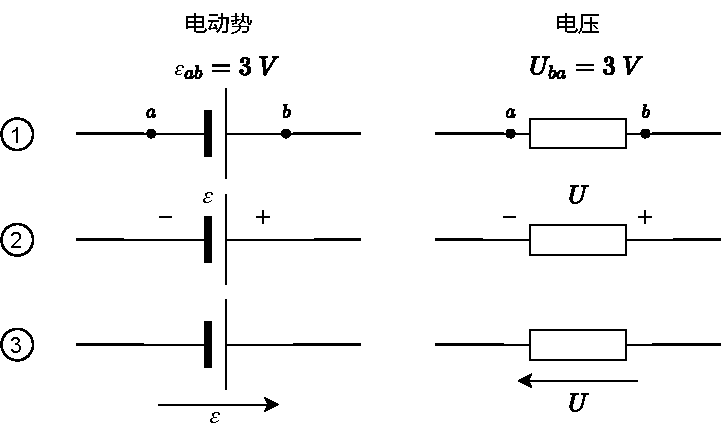
\includegraphics[width=0.45\textwidth]{assets/电动势与电压.drawio.pdf}
\caption{\textbf{电压与电动势的三种表示方法}}\label{电压与电动势的三种表示方法}
\end{figure}

电压、电流定义式:
\begin{equation}
u_{ab} = \frac{\mathrm{d} w_{ab}}{\mathrm{d}q},\ i_{ab} = \frac{\mathrm{d} q_{ab}}{\mathrm{d}t}
\end{equation}

部分常见的电路元件如图 \ref{部分常见电路元件} 所示:

\begin{figure}[H]\centering
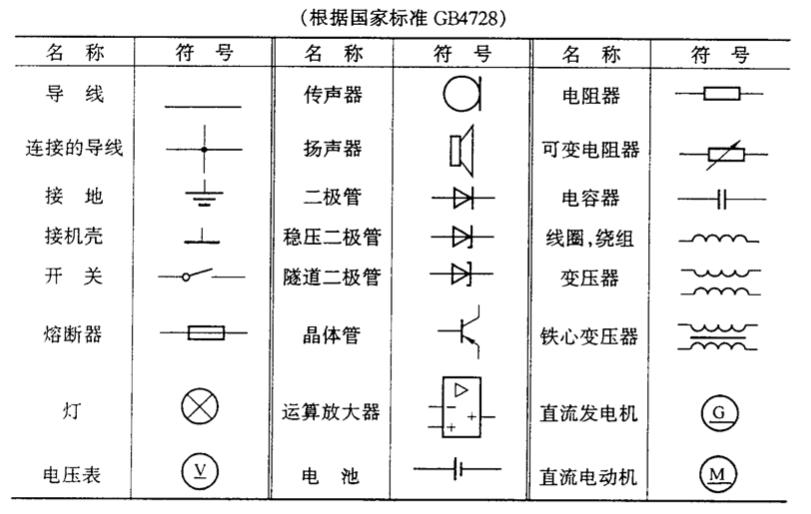
\includegraphics[width=0.5\textwidth]{assets/7d3f6db847882c6447cc046186ede6ef.png}
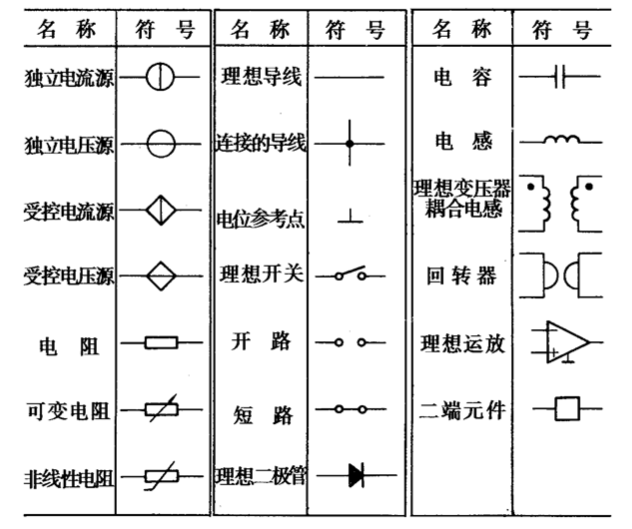
\includegraphics[width=0.5\textwidth]{assets/3f5d73ec5ae9909ab42cd864852b0d72.png}
\caption{\textbf{部分常见电路元件}}\label{部分常见电路元件}
\end{figure}

端口:封装好的电路元件与电路其它部分的联接点称为端纽、端子或接线端(terminal)。如果从元件的两个端纽看进去满足 $i = -i'$,则这两个端子被称为一个端口(port)
\footnote{任意二端电路元件都可以看作是一个端口}
,如图 \ref{端口示意图} 所示。

\begin{figure}[H]\centering

\includegraphics[width=0.33\textwidth]{assets/端口.drawio.png}
\caption{\textbf{端口示意图}}\label{端口示意图}
\end{figure}

与外部电路有 $n$ 个端口相连的电路称为 $n$ 端口网络(n-port network)。

\section{电路分析基本观点}


\begin{definition}[建立电路模型]
电阻、电感与电容:
\begin{equation}
U = RI,\ \varPsi = LI,\ Q = CU
\end{equation}

$R, L, C$ 被称为电路基本模型,是电路分析的最基本模型。对不同的电路,应采用不同的模型,以适应实际需要并满足所需精度。另外,电路中常常使用大量的等效观点来简化电路的分析,使其求解更易、物理意义更清晰、应用更方便。

\end{definition}


\section{电路信号处理}

电路信号可分为 图 \ref{信号分类} 中的几类,它们的示意图如 图 \ref{信号示意图} 所示: 

\begin{figure}[H]\centering
\includesvg[width=0.55\textwidth]{assets/信号分类.drawio.svg}
\caption{\textbf{信号分类}}\label{信号分类}
\end{figure}

\begin{figure}[H]\centering
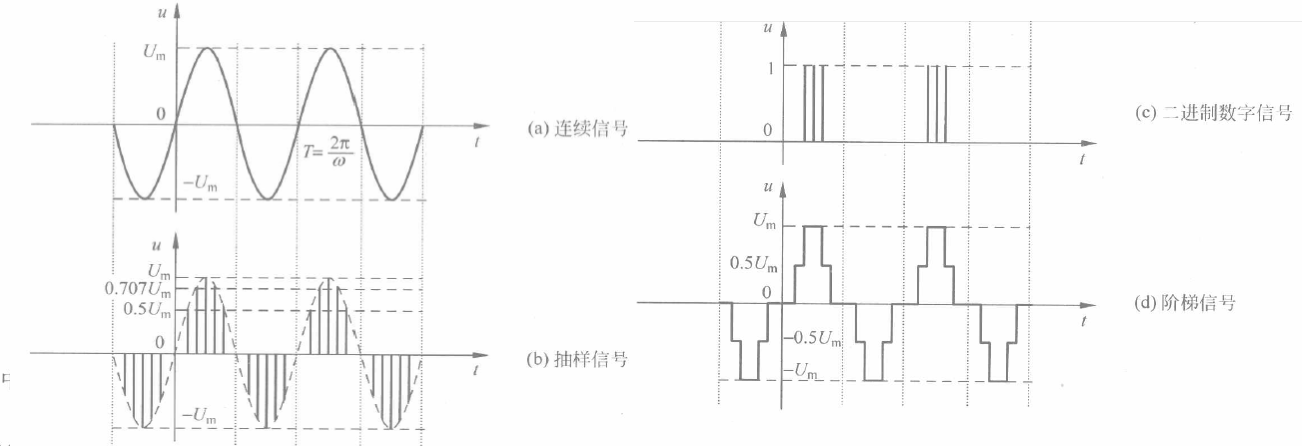
\includegraphics[width=0.75\textwidth]{assets/1b9e0bed85e1f3a049de96f4c6018da8.png}
\caption{\textbf{信号示意图}}\label{信号示意图}
\end{figure}

\section{电路能量处理}


\begin{definition}[功率]

二端元件吸收的瞬时功率(instantaneous power)为其单位时间内吸收的电能\footnote{在非关联参考方向下,吸收的瞬时功率为 $p = -ui$}:
\begin{equation*}
p(t) = \frac{\mathrm{d}w}{\mathrm{d}t} = \frac{\mathrm{d}w}{\mathrm{d}q}\cdot\frac{\mathrm{d}q}{\mathrm{d}t} = u(t)i(t) 
\end{equation*}


\begin{definition}[平均值、有效值]
对周期信号而言,其物理量有瞬时值、平均值、平均绝对值和有效值等特征量。以电压 $u = u(t)$ 为例:

\begin{enumerate}
\item 平均值(average value):$\bar{u} = \frac{1}{T}\int_0^T u(t)\mathrm{d}t$
\item 绝对平均值(average absolute value):$\overline{| u |} = \frac{1}{T}\int_0^T | u(t) |\mathrm{d}t$
\item 有效值(effective value):$ U = \sqrt{\frac{1}{T}\int_0^T u^2(t)\mathrm{d}t} $
\end{enumerate}
电流 $i$ 与上面同理。特别地,对正弦交流电流(sinusoidal altering current)而言,其有效值 $I = \frac{I_{\mathrm{m}}}{\sqrt{2}},\ U = \frac{U_{\mathrm{m}}}{\sqrt{2}}$。
\end{definition}


\end{definition}


\section{电路分类}


\begin{definition}[静态 / 动态电路]
    电路里,将可以提供能量或信号的元件称为源(source),将对能量或信号进行传输、分配和处理的元件称为负载(load)。
    负载全为电阻的电路称为电阻电路或静态电路,否则称为动态电路。前者需求解代数方程组,后者需求解微分方程组。本书第 2~4 章讨论静态电路,第 5~6 章讨论动态电路。
\end{definition}


\begin{definition}[线性 / 非线性电路]
判断是否线性需要先定义系统的激励(excitation)和响应(response),设激励为 $x$ 而响应为 $y = f(x)$,则系统是否线性由 $f$ 决定。例如电阻是二端线性系统,发光二极管是二端非线性系统。
\end{definition}


\begin{definition}[时变 / 非时变电流]
参数随时间变化的元件称为时变元件,含此类元件的电路称为时变电路,否则称为非时变电路。
\end{definition}


\begin{definition}[有源 / 无源电路]
对任意的一端口网络来说,设其端口电压 $u = u(t)$ 且 $u(0) = 0$ ,电流 $i = i(t)$ 且 $i(0) = 0$,该电路称为无源电路如果:
\begin{equation}
\int_{0}^{t} u(t)i(t)\mathrm{d}t \geqslant 0,\ \forall\ t >0
\end{equation}
否则称为有源电路,无源元件和有源元件同理。
\end{definition}


其它还可分为集总 / 分布参数电路、模拟 / 数字电路等。

\section{其它}

\begin{definition}[电路的基本名词]
以图 \ref{电路基本名词} 为例:
\begin{enumerate}
\item 支路:若干元件无分岔地首尾相连构成一条支路。图里有三条支路(竖向的),因此 $p = 3$。
\item 节点(node):3个或更多支路的连接点。图中 $n = 4$。 
\item 路径(path):两个节点间包含的支路个数。
\item 回路(loop):由支路构成的闭合路径。图中 $l = 7$
\item 网格(mesh):平面电路中不与其余支路相交的回路,即最小网格数。图中 $m = 3$
\end{enumerate}

\begin{figure}[H]\centering
\includesvg[width=0.35\textwidth]{assets/电路基本名词.drawio.svg}
\caption{\textbf{电路基本名词}}\label{电路基本名词}
\end{figure}

\end{definition}


\chapter{简单电阻电路}
\section{电阻}
设一均匀线性电阻微元长 $\mathrm{d} l$,横截面积为 $\mathrm{d}S$,电阻率为 $\sigma$,则阻值为
\begin{gather}
    \mathrm{d}R = \frac{\mathrm{d} l}{\sigma\mathrm{d}S} \Longrightarrow R = \frac{L}{\sigma S} = \frac{\rho L}{S} \\
\text{串联:}\ R = \sum_{i}R_i\ , \ \ 
\text{并联:}\ \frac{1}{R} = \sum_{i}\frac{1}{R_i} 
\end{gather}

多数金属材料的电阻率随温度变化见下式,其中 $\alpha$ 称为电阻温度系数,在实际使用时,最好保持额定功率在实际承受功率的两倍以上,以免过载。常见材料的具体数值见表 \ref{常见材料的0度电阻率和温度系数}。
\begin{equation}
\rho(T) = \rho_0(1+\alpha T)
\end{equation}
\begin{table}[H]\centering\small
    \setlength{\tabcolsep}{2mm} % 调整列间距
    \caption{\textbf{常见材料的 0 \textdegree C 电阻率和温度系数 }}
    \label{常见材料的0度电阻率和温度系数}
    \resizebox{\linewidth}{!}{
        \begin{tabular}{cccccccccc}\toprule
            名称 & 银 & 铜 & 铝 & 钨 & 铁 & 碳 & 镍铬合金 & 镍铜合金\\
            \midrule
            $\rho_0\ (\Omega\cdot \mathrm{m})$
            &$1.5 \times 10^{-8}$ 
            &$1.6 \times 10^{-8}$ 
            &$2.5 \times 10^{-8}$ 
            &$2.5 \times 10^{-8}$ 
            &$8.7 \times 10^{-8}$ 
            &$3500 \times 10^{-8}$ 
            &$110 \times 10^{-8}$ 
            &$50 \times 10^{-8}$ \\
            $\alpha\ (\text{\textdegree C}^{-1})$
            &$4.0 \times 10^{-3}$ 
            &$4.3 \times 10^{-3}$ 
            &$4.7 \times 10^{-3}$ 
            &$4.6 \times 10^{-3}$ 
            &$5.0 \times 10^{-3}$ 
            &$-5.0 \times 10^{-4}$ 
            &$1.6 \times 10^{-4}$ 
            &$4.0 \times 10^{-5}$ \\
            \bottomrule
        \end{tabular}
    }
\end{table}


我们有欧姆定律微分形式和焦耳定律微分形式
\begin{equation}
i = \sigma E\ ,\ \ q =  \sigma E^2 = \frac{1}{\sigma} i^2  
\end{equation}

二极管模型:
\begin{equation}
i = I_{\mathrm{S}}\left(e^{\frac{u}{U_{\mathrm{TH}}}} - 1\right)
\end{equation}
其中 $I_{\mathrm{S}}$ 为反向饱和电流(硅二极管的典型值为 $10^{-12}$ A),$U_{TH}$ 为常数(典型值 25 mV)。

伏安特性曲线($u$-$i$ 特性曲线,voltage current relationship,VCR)的表达式为 $i = f(u)$ 或 $f(u,i) = 0$,
到目前为止,我们讨论的电阻 $u$-$i$ 特性曲线都在平面的一三象限(正电阻),后文我们将在等效观念指导下用运算放大器来实现负电阻性质。

\section{电源}


\begin{definition}[独立电源]
与外接电路无关的二端电源称为独立电源(independent source),例如独立电压源(independent voltage source)和独立电流源(independent current source)
\footnote{电压为零的独立电压源等效于短路,电流为零的独立电流源等效于断路}。
\end{definition}


\begin{definition}[受控电源]

流经元件的电压或电流受电路中其它部分电压或电流控制的元件称为受控电源。最常见的例子是放大器,如电子管、晶体管(又称三极管)等。
依据控制量和受控量的不同,受控电源一般分为 4 种:
    \begin{itemize}
    \item 压控电压源(voltage controlled voltage source, VCVS)
    \item 流控电压源(current controlled voltage source, CCVS)
    \item 压控电流源(voltage controlled current source, VCCS)
    \item 流控电流源(current controlled current source, CCCS)
    \end{itemize}
它们的电路符号如图 \ref{受控电源电路符号} 所示。 

\begin{figure}[H]\centering
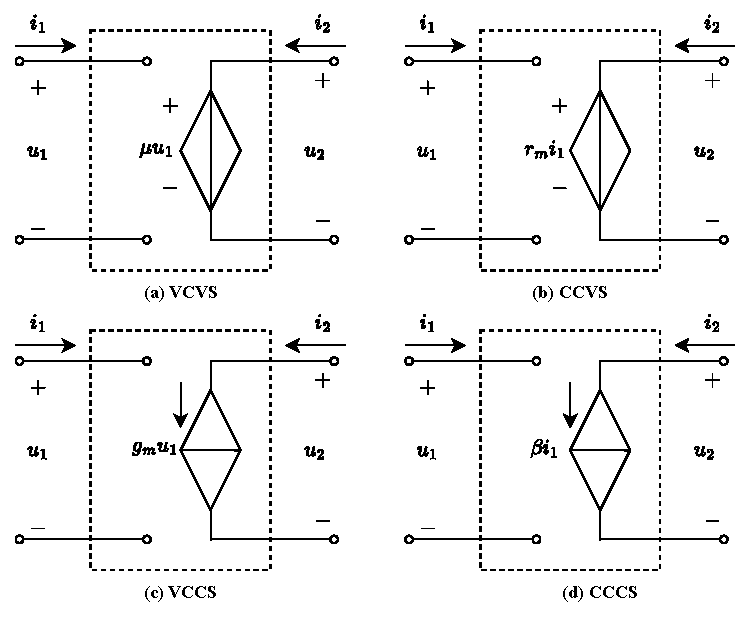
\includegraphics[width=0.7\textwidth]{assets/受控电源电路符号.drawio.pdf}
\caption{\textbf{受控电源电路符号}}\label{受控电源电路符号}
\end{figure}

图 \ref{受控电源电路符号} 中,控制量 $u_1$ 和 $i_1$ 分别是电路其它部分任意两点间的电压或电流;$\mu$ 是一个无量纲常数,称为电压放大倍数(转移电压比);$r_m$ 是电阻量纲常数,称为转移电阻;$g_m$ 是电导量纲常数,称为转移电导;$\beta$ 是无量纲常数,称为电流放大倍数(转移电流比)。

分析含受控源电路时需要注意,受控源性质和独立源有本质差别,不应简单等同。
\end{definition}


\section{MOSFET(金属氧化物半导体场效应晶体管)}
\noindent % 避免第一栏内容产生缩进  
\begin{minipage}[t]{0.69\textwidth} % 左栏  

\hspace{2em} MOSFET standing for ``metal oxide semiconductor field effect transistor'',右图是一个 N MOSFET 的示意图,三个端纽分别称为栅极 G、源级 S 和漏级 D。

\hspace{2em} 由于 MOSFET 结构上的特点,没有电流流经栅极 G,因此可以把 D-S 看作一个二端元件,研究其伏安特性曲线 VCR。栅极和源级之间的电压 $u_{GS}$ 会对 VCR 产生影响,主要表现为 D-S 开路或非开路。N MOS 管可视为一个非线性的 VCVS。

\hspace{2em} 使得 D-S 之间不再开路的电压阈值称为阈值电压,记为 $U_T$(典型值为 1 V)。对一个非开路的 D-S VCR,大致可分为两段:电阻区(斜线区)和恒流区(水平线区)。
\end{minipage}%  
\hfill % 填充空白以使两栏间无间隙  
\begin{minipage}[t]{0.3\textwidth} % 右栏  
\begin{figure}[H]\centering
    \includesvg[width=\textwidth]{assets/MOS管符号.drawio.svg}
    \caption{\textbf{N MOS 示意图}}\label{N MOS 示意图}
\end{figure}
\end{minipage}\vfill

可以证明,$u_{\mathrm{GS}}$ 和 $i_{\mathrm{DS}, max}$ 是非线性关系。其中 $K$ 为常数(典型值 1 $\mathrm{mA V^{-2}}$),$U_{\mathrm{T}}$ 为阈值电压。
\begin{equation}
    i_{\mathrm{DS}, max} = \frac{K}{2}(u_{\mathrm{GS}} - U_{\mathrm{T}})^2
\end{equation}



\section{基尔霍夫定律}


\begin{BlockTheorem}[基尔霍夫电流定律, KCL]
基尔霍夫电流定律(Kirchhoff's Current Law,KCL)表示,在任意时刻,电路中流入任一节点的电流代数和都为 0。
\begin{equation}
\sum i(t) = 0,\ \forall\ t 
\end{equation}
KCL 不仅适用于节点,对含多个端子的子电路也适用,称为广义 KCL。此定律本质上是是电流连续性 $\frac{\mathrm{d}q}{\mathrm{d}t} = 0$。

$n$ 节点电路含 $n-1$ 个独立的电流节点方程,构成第一方程组。
\end{BlockTheorem}

\begin{BlockTheorem}[基尔霍夫电压定律, KVL]
基尔霍夫电压定律(Kirchhoff's Voltage Law,KVL)表示,在任意时刻,沿任意回路的电压降(代数和)为 0。
\begin{equation}
\sum u(t) = 0,\ \forall\ t
\end{equation}
此定律本质上是法拉第电磁感应定律 $\oint \boldsymbol{E} \mathrm{d}\boldsymbol{l} = -\frac{\p \phi_B}{\p t} = 0$。

$n$ 节点 $p$ 支路的电路含有 $p-n+1$ 个独立的回路方程(即最小网格数),构成第二方程组。
\end{BlockTheorem}


\section{电路等效变换}

\subsection{电阻等效变换}

\begin{definition}[平衡电桥]

如 图 \ref{平衡电桥},当 $\frac{R_1}{R_2} = \frac{R_3}{R_4}$ 时,$\varphi_A = \varphi_B$,AB 段无电流通过。 

\begin{figure}[H]\centering
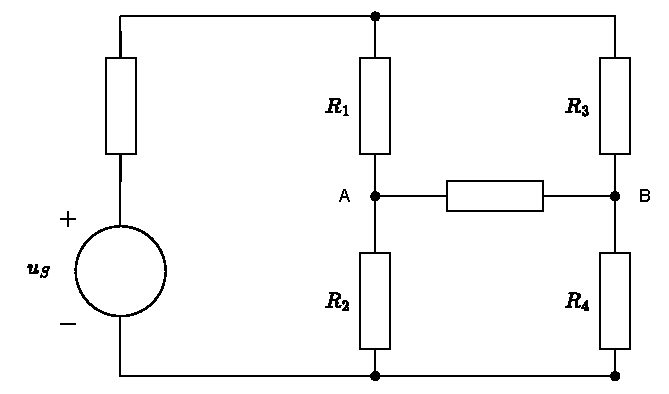
\includegraphics[width=0.43\textwidth]{assets/平衡电桥.drawio.pdf}
\caption{\textbf{平衡电桥}}\label{平衡电桥}
\end{figure}

\end{definition}


\begin{definition}[Y-$\Delta$ 等效变换]

已知 Y 型,求 $\Delta$ 型:
\begin{equation}
\begin{aligned}
    R_{12}&=\frac{1}{R_{3}}(R_{1}R_{2}+R_{1}R_{3}+R_{2}R_{3})\\
    R_{13}&=\frac{1}{R_{2}}(R_{1}R_{2}+R_{1}R_{3}+R_{2}R_{3})\\
    R_{23}&=\frac{1}{R_{1}}(R_{1}R_{2}+R_{1}R_{3}+R_{2}R_{3})
\end{aligned}
\end{equation}

已知 $\Delta$ 型,求 Y 型:、
\begin{equation}
\begin{aligned}
    R_{1}&=\frac{R_{12}R_{13}}{R_{12}+R_{13}+R_{23}}\\
    R_{2}&=\frac{R_{21}R_{23}}{R_{12}+R_{13}+R_{23}}\\
    R_{3}&=\frac{R_{31}R_{32}}{R_{12}+R_{13}+R_{23}}
\end{aligned}
\end{equation}

\begin{figure}[H]\centering
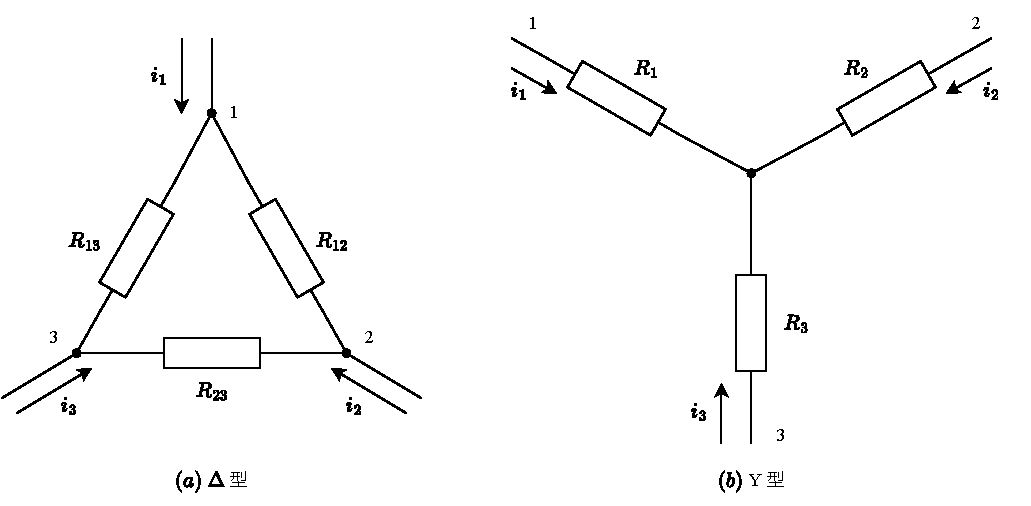
\includegraphics[width=0.65\textwidth]{assets/YDelta等效变换.drawio.pdf}
\caption{\textbf{Y-$\Delta$ 等效变换}}\label{Y-Delta等效变换}
\end{figure}
\end{definition}

\subsection{电源等效变换}

含电阻和受控源的二端网络一般可等效为一个电阻。由于电路性质只与电路内部结构和参数有关,与外接激励无关,因此无论是外接独立电压源,还是外接独立电流源,都可以求出等效电阻。


\begin{definition}[独立源等效替换]
如图 \ref{实际独立源等效示意图},当满足下式时,两者可以等效替换。
\begin{equation}
U_S = I_SR_S\ \  \text{或}\ \  I_S = \frac{U_S}{R_S}
\end{equation}

\begin{figure}[H]\centering
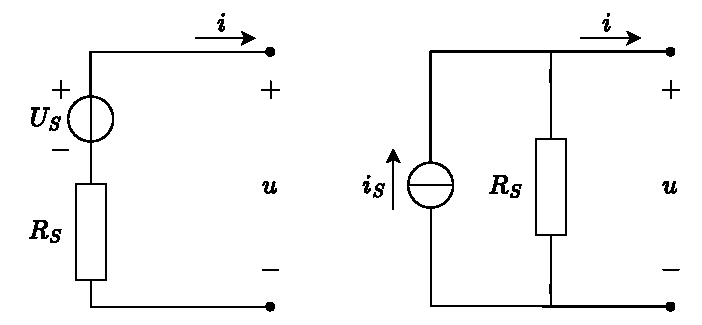
\includegraphics[width=0.5\textwidth]{assets/独立源等效.drawio.pdf}
\caption{\textbf{实际独立源等效示意图}}\label{实际独立源等效示意图}
\end{figure}

例如,将电流源等效为电压源时,保持 $R_S$ 不变,令 $U_S = I_S R_S$ 即可;将电压源等效为电流源时,保持 $R_S$ 不变,令 $I_S = \frac{U_S}{R_S}$ 即可。
\end{definition}


\begin{definition}[最大功率传输]
大多数仅含独立源和线性电阻的电路都可等效为一个实际独立电压源(内阻 $R_S$)外接一个负载电阻 $R_L$,则当且仅当 $R_S = R_L$ 时,$R_L$ 有最大功率。
\begin{equation}
P_L = P_L(R_L) =  \left(\frac{U_S}{R_S + R_L}\right)^2R_L, \ P_{L,\mathrm{max}} = P_L(R_S) = \frac{U_S^2}{4R_S}
\end{equation}
\end{definition}


\section{运算放大器}
运算放大器(operational amplifier, Op Amp, OPA),简称运放,是一种性质特殊的多端集成电路,可视为电压放大器。借助 OPA,可实现模拟信号的各种数学运算。

在图 \ref{OPA 示意图} 中,OPA 的国标电路符号如图 (a) 所示,简化符号如图 (b) 所示,过去也惯用符号图 (c)。
\begin{figure}[H]\centering
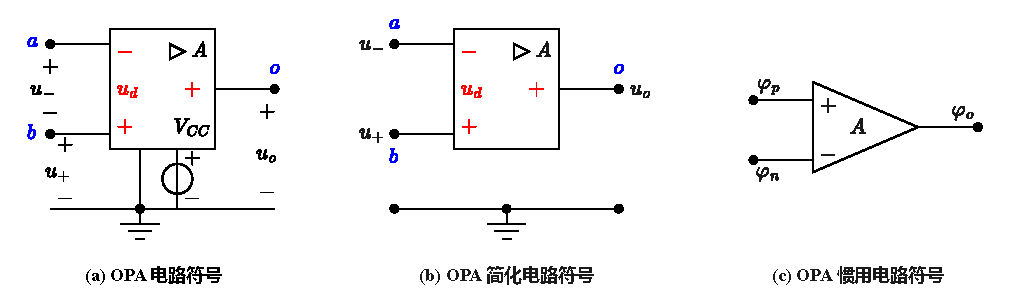
\includegraphics[width=0.8\textwidth]{assets/OPA运放.drawio.pdf}
\caption{\textbf{OPA 示意图}}\label{OPA 示意图}
\end{figure}

其中,a 接线端称为反相输入端(inverting input),用 $u_-$ 表示;b 接线端称为同相输入端(noninverting input),用 $u_+$ 表示;o 接线端称为输出端(output),用 $u_o$ 表示; $V_{CC}$ supply voltage, working voltage),向 OPA 提供直流电压以保证其正常工作;接地端 ground 并非大地,而是电源 $V_{CC}$ 的公共参考零点;参数 $A$ 为开环放大倍数。

需要注意,在图 \ref{OPA 示意图} (b) 中,因为省略了电源部分,所以包围 OPA 的封闭曲线不满足广义 KCL。

OPA 的主要电气参数包括:

\begin{enumerate}
\item 供电电压(supply voltage)$V_{CC}$
\item 开环电压增益(open-loop voltage gain)$A$:在开环情况下(无输入引回到输出)满足
\begin{equation}
    u_o = A(u_+-u_-) = Au_d
\end{equation}
\end{enumerate}


\subsection{运算放大器及其电气特性}


\section{二端口网络}
\section{数字系统}
\section{门电路}

\chapter{线性电阻电路}
\section{支路电流法}
\section{节点电压法}
\section{回路电流法}
\section{叠加定理与齐性定理}
\section{替代定理}
\section{戴维南定理和诺顿定理}
\section{特勒根定理}
\section{互易定理}
\section{对偶电路和对偶原理}





































































































































































































































































































































































































































































\nocite{*}
\bibliography{re}
\thispagestyle{fancy} 
\addcontentsline{toc}{chapter}{参考文献}




\newpage
\appendix
\titlespacing*{\chapter}{0pt}{-15pt}{8pt} % 控制上方空白的大小
\titleformat{\section}{\large\centering\bfseries}{\thesection}{1em}{}
\titleformat{\subsection}{\normalsize\bfseries}{\thesubsection}{1em}{}

\chapter*{附录 A: 中英文对照表}\addcontentsline{toc}{chapter}{附录 A: 中英文对照表}\thispagestyle{fancy} 
\begin{multicols}{2}  
\begin{table}[H]\centering
\caption{\textbf{中英文对照表}}
\begin{tabular}{cccccccc}\toprule
    English & 中文 \\
    \midrule
    voltage            & 电压 \\
    current            & 电流 \\
    power              & 功率 \\
    resistance         & 电阻 \\
    conductance        & 电导 \\
    inductance         & 电感 \\
    capacitance        & 电容 \\
    resistor           & 电阻器 \\
    capacitor          & 电容器 \\
    inductor           & 电感器 \\
    frequency          & 频率 \\
    circuit            & 电路 \\
    circuit element    & 电流元件 \\
    signal             & 信号 \\
    circuit analysis   & 电路分析 \\
    circuit synthesis  & 电路综合 \\
    circuit design     & 电路设计 \\
    circuit topology   & 电路拓扑 \\
    electromotive force, e.m.f. & 电动势 \\
    potential & 电势 \\
    reference point & 参考点 \\
    potential rise & 电势升 \\
    potential drop & 电势降 \\
    terminal & 端纽,接线端\\ 
    source & 源 \\
    load & 负载 \\
    independent source & 独立源 \\ 
    independent voltage source & 独立电压源 \\ 
    independent current source & 独立电流源 \\ 
    excitation & 激励 \\
    response & 响应 \\
    n-port network & n 端口网络 \\
    instantaneous power & 瞬时功率 \\
    average value & 平均值 \\
    average absolute value & 绝对平均值 \\
    effective value & 有效值 \\
    \bottomrule
\end{tabular}
\end{table}

\begin{table}[H]\centering
    \caption{\textbf{中英文对照表}}
    \begin{tabular}{cccccccc}\toprule
        English & 中文 \\
        \midrule
        sinusoidal altering current & 正弦交流电流 \\
        \bottomrule
    \end{tabular}
    \end{table}




\end{multicols} 






















\end{document}



% VScode 常用快捷键:

% F2:                       变量重命名
% Ctrl + Enter:             行中换行
% Alt + up/down:            上下移行
% 鼠标中键 + 移动:           快速多光标
% Shift + Alt + up/down:    上下复制
% Ctrl + left/right:        左右跳单词
% Ctrl + Backspace/Delete:  左右删单词    
% Shift + Delete:           删除此行
% Ctrl + J:                 打开 VScode 下栏(输出栏)
% Ctrl + B:                 打开 VScode 左栏(目录栏)
% Ctrl + `:                 打开 VScode 终端栏
% Ctrl + 0:                 定位文件
% Ctrl + Tab:               切换已打开的文件(切标签)
% Ctrl + Shift + P:         打开全局命令(设置)

% Latex 常用快捷键

% Ctrl + Alt + J:           由代码定位到PDF
% 


% Git提交规范:
% update: Linear Algebra 2 notes
% add: Linear Algebra 2 notes
% import: Linear Algebra 2 notes
% delete: Linear Algebra 2 notes














































































































































































































































































































































































































































































































































































































\end{document}

% VScode 常用快捷键:

% F2:                       变量重命名
% Ctrl + Enter:             行中换行
% Alt + up/down:            上下移行
% 鼠标中键 + 移动:           快速多光标
% Shift + Alt + up/down:    上下复制
% Ctrl + left/right:        左右跳单词
% Ctrl + Backspace/Delete:  左右删单词    
% Shift + Delete:           删除此行
% Ctrl + J:                 打开 VScode 下栏(输出栏)
% Ctrl + B:                 打开 VScode 左栏(目录栏)
% Ctrl + `:                 打开 VScode 终端栏
% Ctrl + 0:                 定位文件
% Ctrl + Tab:               切换已打开的文件(切标签)
% Ctrl + Shift + P:         打开全局命令(设置)

% Latex 常用快捷键

% Ctrl + Alt + J:           由代码定位到PDF
% 


% Git提交规范:
% update: Linear Algebra 2 notes
% add: Linear Algebra 2 notes
% import: Linear Algebra 2 notes
% delete: Linear Algebra 2 notes
